\begin{figure}[htbp]
    \centering
    \begin{subfigure}[b]{0.49\textwidth}
       \centering
       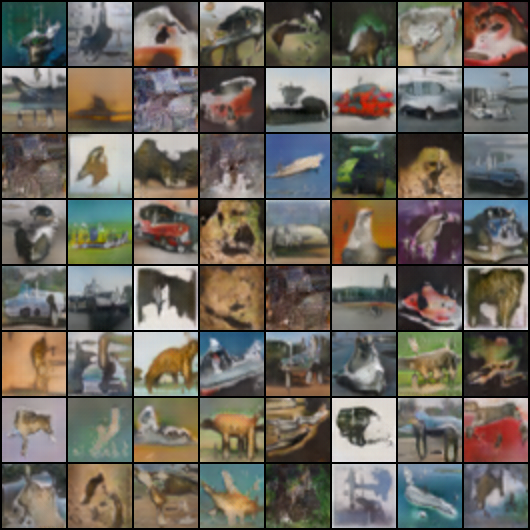
\includegraphics[width=\exfactor\textwidth]{figures/cifar/192_base_raw_base.png}
       \caption{GAN}
    \end{subfigure}
    \begin{subfigure}[b]{0.49\textwidth}
       \centering
       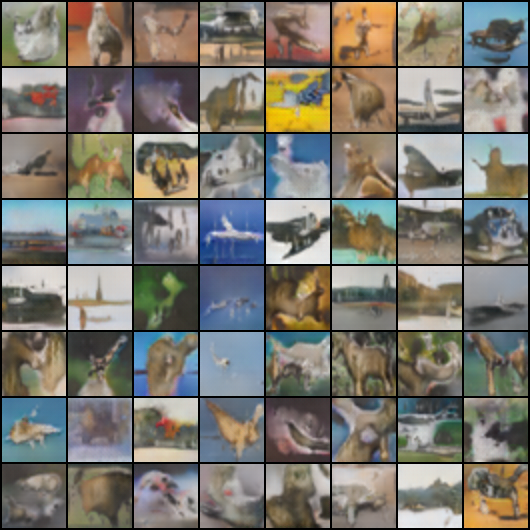
\includegraphics[width=\exfactor\textwidth]{figures/cifar/192_base_raw_reject.png}
       \caption{DRS}
    \end{subfigure}
    \begin{subfigure}[b]{0.49\textwidth}
       \centering
       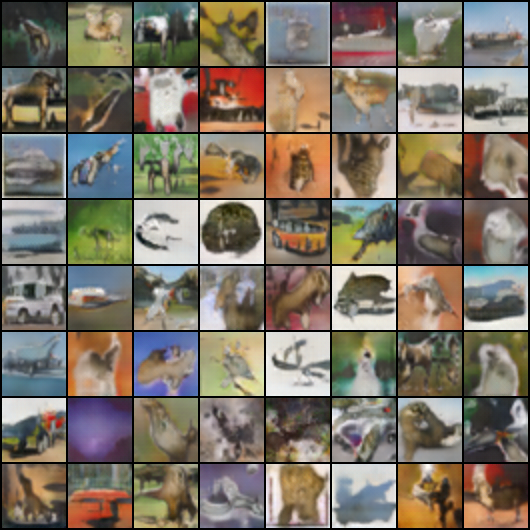
\includegraphics[width=\exfactor\textwidth]{figures/cifar/192_base_raw_MH.png}
       \caption{MH-GAN}
    \end{subfigure}
    \begin{subfigure}[b]{0.49\textwidth}
       \centering
       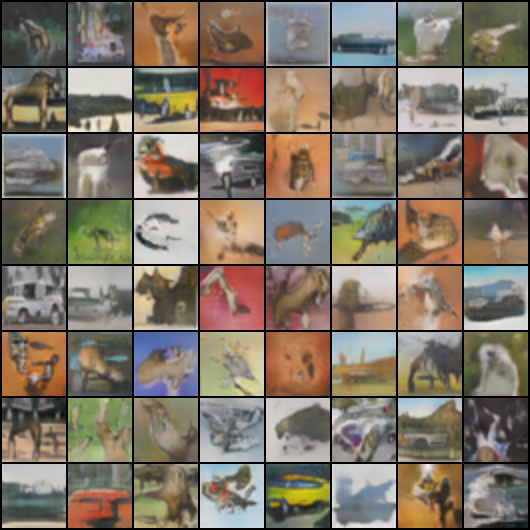
\includegraphics[width=\exfactor\textwidth]{figures/cifar/192_base_iso_MH.png}
       \caption{MH-GAN (cal)}
    \end{subfigure}
    \caption{{\small
    Example images on CIFAR-10 for different GAN setups.
    The different selectors (MH-GAN and DRS) are run on the same batch of images.
    Meaning, the same images may appear for both generators.
    The calibrated MH-GAN shows a greater preference for animal-like images with four legs.
    }}
    \label{fig:cifar_samples}
\end{figure}

